\chapter{Resultate}\label{chap:r} 

Die Resultate tragen die in der Testumgebung erfassten Daten und Werte über die
KI zusammen. Für die verschiedenen Variationen und Kriterien werden nachfolgend
Abkürzungen eingeführt, die für die Präsentation und die Diskussion der
Resultate fortan verwendet werden.

Die Abkürzungen der Kriterien lauten:
\begin{itemize}
    \item Sim (siehe \doubleref{sub:m_eval_proc})
    \item Rec (siehe \doubleref{sub:m_eval_rec})
    \item Speed (siehe \doubleref{sub:m_eval_speed})
    \item Drawtime  (siehe \doubleref{sub:m_eval_zeichnend})
    \item Overdrawn (siehe \doubleref{sub:m_eval_uebermalung})
\end{itemize}

Die Abkürzungen der Variationen der nachzeichnenden KI lauten: 
\begin{itemize}
    \item Base (siehe \doubleref{sub:m_var_base})
    \item Rec (siehe \doubleref{sub:m_var_rec})
    \item Speed (siehe \doubleref{sub:m_var_speed})
    \item No-Penlift (+ Speed) (siehe \doubleref{sub:m_var_penlift})
    \item No-Overdraw (siehe \doubleref{sub:m_var_overdraw})
    \item Physics (siehe \doubleref{sub:m_var_phy})
\end{itemize}

Die Abkürzungen der Variationen der generativen KI lauten:
\begin{itemize}
    \item Softmax (siehe \doubleref{sub:m_gen_det})
    \item Random-Noise (siehe \doubleref{sub:m_gen_det})
\end{itemize}



\section{Tabellen}\label{chap:r_tab} 

Der erste Teil der Resultate besteht aus Tabellen, welche die Daten über die
Leistung der KI aus der Testumgebung (siehe \doubleref{chap:m_auswert})
zusammentragen. Die Tabellen sind dabei in diejenigen der nachzeichnenden KI und
diejenigen der generativen KI unterteilt.

\subsection{Tabellen der nachzeichnenden KI}\label{sub:r_tab_nachzeich}
Die Tabellen für die nachzeichnende KI beschreiben die Leistung jeder Variation
in jedem Kriterium. Es gibt insgesamt drei Tabellen für die nachzeichnende KI.
Der Unterschied in den Tabellen liegt im Datenset, mit denen die KI jeweils
getestet wurde.

\begin{table}[!ht]
    \centering
    \caption{Testen auf MNIST Datenset | 1000 Tests}\label{tab:MNIST}
    \begin{tabular}{|l|l|l|l|l|l|}
            \hline
            \hline ~ & Sim $[\%]$ & Rec $[\%]$ & Speed & Drawtime $[\%]$ & Overdrawn \\ \hline
            Base & 0 & 0 & 0 & 0 & 0 \\ \hline
            Rec & 0 & 0 & 0 & 0 & 0 \\ \hline
            Speed & 0 & 0 & 0 & 0 & 0 \\ \hline
            No-Penlift & 0 & 0 & 0 & 0 & 0 \\ \hline
            No-Overdraw & 0 & 0 & 0 & 0 & 0 \\ \hline
            Physics & 0 & 0 & 0 & 0 & 0 \\ \hline
        \end{tabular}
\end{table}

\begin{table}[!ht]
    \centering
    \caption{Testen auf EMNIST Letters Datenset | 1000 Tests}\label{tab:EMNIST}
    \begin{tabular}{|l|l|l|l|l|l|}
        \hline ~ & Sim $[\%]$ & Rec $[\%]$ & Speed & Drawtime $[\%]$ & Overdrawn \\ \hline
        Base & 0 & 0 & 0 & 0 & 0 \\ \hline
        Rec & 0 & 0 & 0 & 0 & 0 \\ \hline
        Speed & 0 & 0 & 0 & 0 & 0 \\ \hline
        No-Penlift & 0 & 0 & 0 & 0 & 0 \\ \hline
        No-Overdraw & 0 & 0 & 0 & 0 & 0 \\ \hline
        Physics & 0 & 0 & 0 & 0 & 0 \\ \hline
    \end{tabular}
\end{table}

\begin{table}[!ht]
    \centering
    \caption{Testen auf QuickDraw Datenset | 1000 Tests}\label{tab:Quickdraw}
    \begin{tabular}{|l|l|l|l|l|l|}
        \hline ~ & Sim $[\%]$ & Rec $[\%]$ & Speed & Drawtime $[\%]$ & Overdrawn \\ \hline
        Base & 0 & 0 & 0 & 0 & 0 \\ \hline
        Rec & 0 & 0 & 0 & 0 & 0 \\ \hline
        Speed & 0 & 0 & 0 & 0 & 0 \\ \hline
        No-Penlift & 0 & 0 & 0 & 0 & 0 \\ \hline
        No-Overdraw & 0 & 0 & 0 & 0 & 0 \\ \hline
        Physics & 0 & 0 & 0 & 0 & 0 \\ \hline
    \end{tabular}
\end{table}


\subsection{Tabellen der generativen KI}\label{sub:r_tab_gen} Die Tabellen der
generativen KI beschreiben die Leistung der beiden Variationen auf die
ausgewählten Kriterien. Für beide Variationen gibt es eine Tabelle, die jeweils
die Leistung dieser Variation für die fünf verschiedenen Motive (siehe
\doubleref{sub:m_auswert_gen}). beschreibt. 


\begin{table}[!ht]
    \centering
    \caption{Testen der Softmax Variation | 1000 Tests}\label{tab:gen-softmax}
    \begin{tabular}{|l|l|l|l|}
    \hline
        ~ & Rec $[\%]$ & Speed & Drawtime $[\%]$ \\ \hline
        Null & 0 & 0 & 0 \\ \hline
        Zwei & 0 & 0 & 0 \\ \hline
        Acht & 0 & 0 & 0 \\ \hline
        F & 0 & 0 & 0 \\ \hline
        Auge & 0 & 0 & 0 \\ \hline
    \end{tabular}
\end{table}

\begin{table}[!ht]
    \centering
    \caption{Testen der Noisy-Pixel Variation | 1000 Tests}\label{tab:gen-noisy}
    \begin{tabular}{|l|l|l|l|}
    \hline
        ~ & Rec $[\%]$ & Speed & Drawtime $[\%]$ \\ \hline
        Null & 0 & 0 & 0 \\ \hline
        Zwei & 0 & 0 & 0 \\ \hline
        Acht & 0 & 0 & 0 \\ \hline
        F & 0 & 0 & 0 \\ \hline
        Auge & 0 & 0 & 0 \\ \hline
    \end{tabular}
\end{table}




\section{Bildersammlung}\label{chap:r_bild} Eine Sammlung von gezeichneten
Strichbildern von ausgewählten Variationen ergänzt die Resultate. Die Zeichnungen, die in der Sammlung
vertreten sind, stammen aus einer zufälligen Auswahl aus dem Test der jeweiligen
Variation der KI. Die Bilder haben einen Farbverlauf, der den zeitliche Verlauf
des Zeichnens darstellt. Die Helligkeit eines Striches ist proportional zu dem
Step, in dem dieser gezeichnet wurde. Das bedeutet, dass dunklere Striche früher
gezeichnet wurden als hellere Striche. Bewegungen des Agents, in denen dieser
nicht zeichnete, sind in den Bildern nicht erkennbar.


\subsection{Bildersammlung der nachzeichnenden KI}\label{sub:r_bild_nach}

Die Strichbilder für die Bildersammlung der nachzeichnenden KI sind jeweils in Paaren
angeordnet. Das linke Bild im Paar zeigt die Vorlage aus dem Datenset und das
rechte Bild zeigt die nachgezeichnete Variante von der KI. Jede Spalte der
Bildersammlung zeigt Bilder aus einem anderen Datenset

\begin{figure}[!ht]
    \centering
    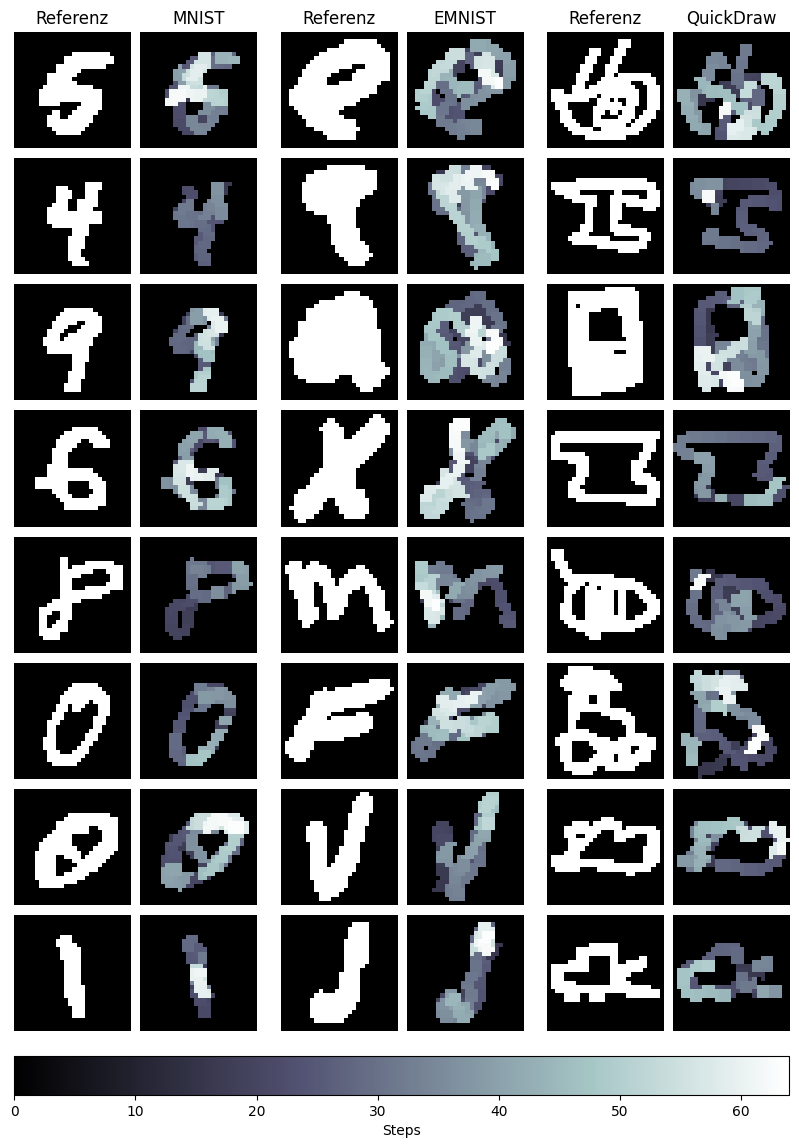
\includegraphics[width=\textwidth]{images/resultate/base.png}
    \caption{Bildersammlung: Base Variation}\label{fig:r-base}
\end{figure}

\begin{figure}[!ht]
    \centering
    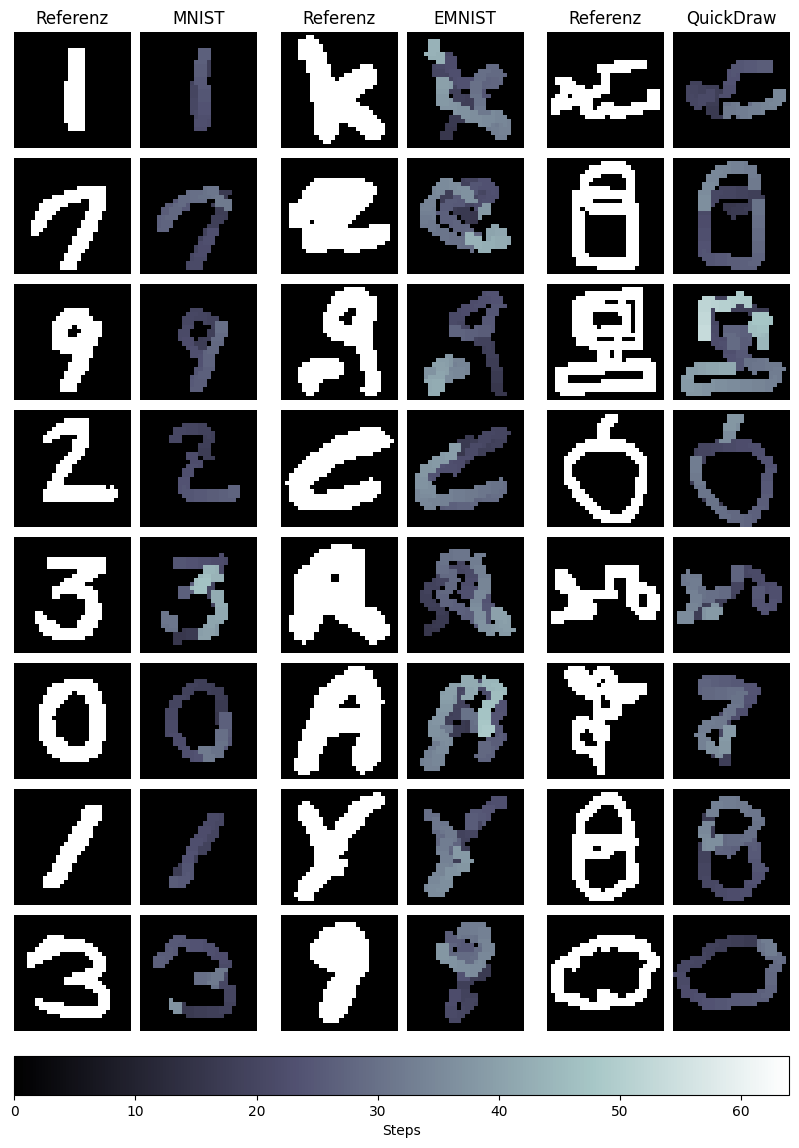
\includegraphics[width=\textwidth]{images/resultate/speed.png}
    \caption{Bildersammlung: Speed Variation}\label{fig:r-speed}
\end{figure}

\begin{figure}[!ht]
    \centering
    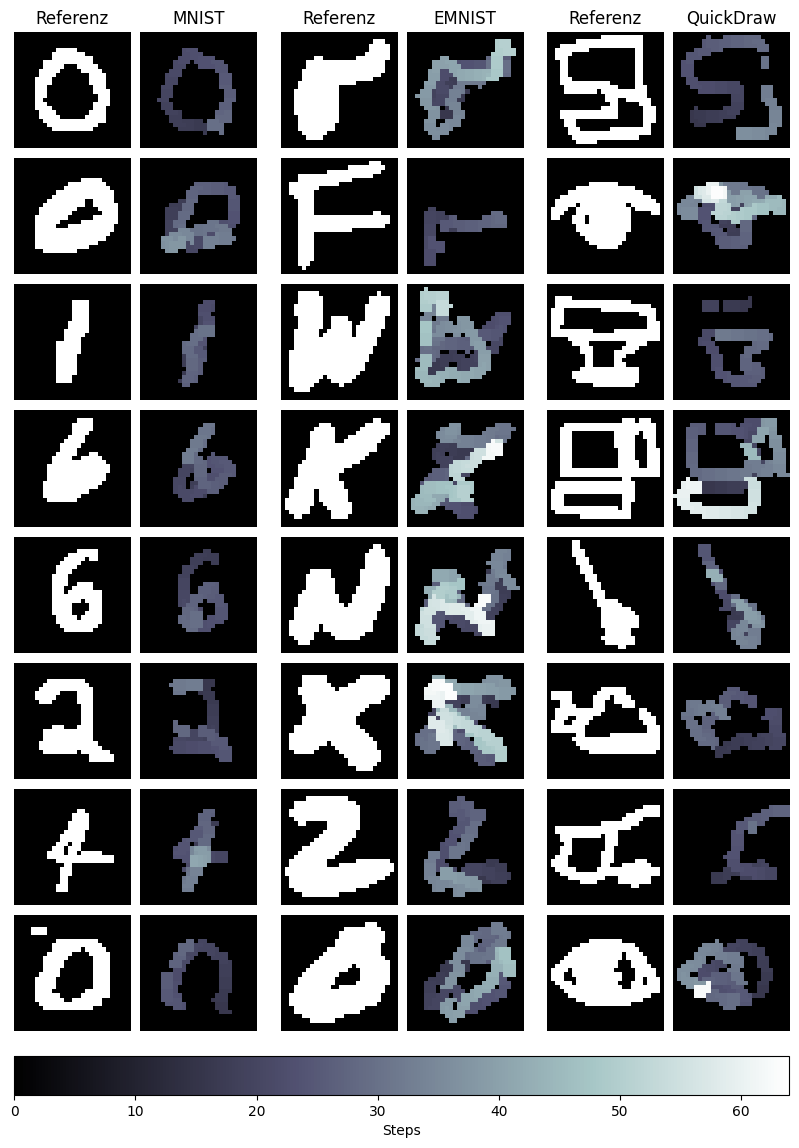
\includegraphics[width=\textwidth]{images/resultate/rec.png}
    \caption{Bildersammlung: Rec Variation}\label{fig:r-rec}
\end{figure}

\begin{figure}[!ht]
    \centering
    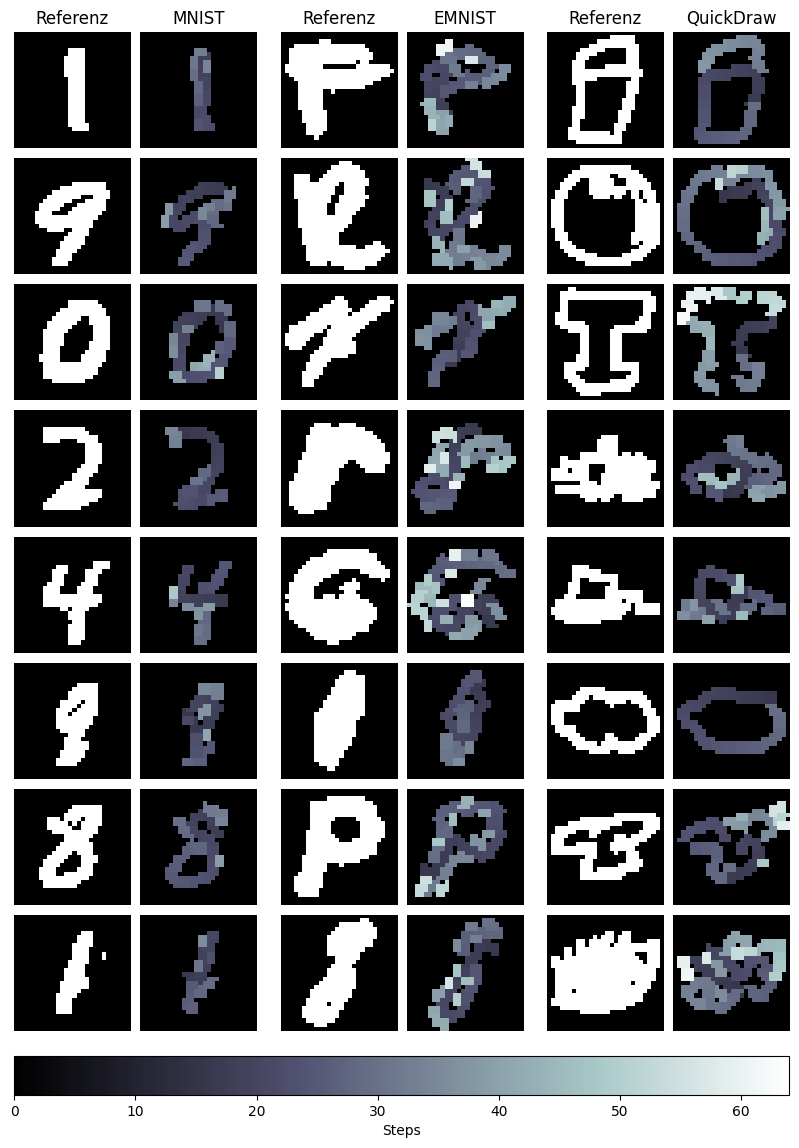
\includegraphics[width=\textwidth]{images/resultate/overdraw.png}
    \caption{Bildersammlung: Overdraw Variation}\label{fig:r-overdraw}
\end{figure}



\subsection{Bildersammlung der generativen KI}\label{sub:r_bild_gen}

Die Bildersammlungen für die Variationen der generativen KI haben fünf Spalten. Jede
Spalte zeigt Zeichnungen der KI von einem der ausgewählten Motive (siehe
\doubleref{sub:m_auswert_gen}).
